\documentclass[12pt, twoside]{article}
\documentclass[12pt, twoside]{article}
\usepackage[letterpaper, margin=1in, headsep=0.2in]{geometry}
\setlength{\headheight}{0.6in}
%\usepackage[english]{babel}
\usepackage[utf8]{inputenc}
\usepackage{microtype}
\usepackage{amsmath}
\usepackage{amssymb}
%\usepackage{amsfonts}
\usepackage{siunitx} %units in math. eg 20\milli\meter
\usepackage{yhmath} % for arcs, overparenth command
\usepackage{tikz} %graphics
\usetikzlibrary{quotes, angles}
\usepackage{graphicx} %consider setting \graphicspath{{images/}}
\usepackage{parskip} %no paragraph indent
\usepackage{enumitem}
\usepackage{multicol}
\usepackage{venndiagram}

\usepackage{fancyhdr}
\pagestyle{fancy}
\fancyhf{}
\renewcommand{\headrulewidth}{0pt} % disable the underline of the header
\raggedbottom
\hfuzz=2mm %suppresses overfull box warnings

\usepackage{hyperref}
\usepackage{float}

\title{Algebra 2}
\author{Chris Huson}
\date{April 2024}

\fancyhead[LE]{\thepage}
\fancyhead[RO]{\thepage \\ Name: \hspace{3cm} \,\\}
\fancyhead[LO]{BECA / Huson / Algebra 2: Exponentials Jan 2023 Regents \\* 18 April 2024}

\begin{document}

\subsubsection*{Regents problems: Exponential functions}
\begin{enumerate}[itemsep=0.5cm]
\item The value of an automobile $t$ years after it was purchased is given by the function $V = 38,000(0.84)^t$. Which statement is true? %January 2023 Regents
\begin{enumerate}
    \item The value of the car increases 84\% each year.
    \item The value of the car decreases 84\% each year.
    \item The value of the car increases 16\% each year.
    \item The value of the car decreases 16\% each year.
\end{enumerate}

\item Which function represents exponential decay? %January 2023 Regents
\begin{enumerate}
    \item $\displaystyle p(x) = \left(\frac{1}{4}\right)^{-x}$
    \item $q(x) = 1.8^{-x}$
    \item $r(x) = 2.3^{2x}$
    \item $s(x) = 4^{\frac{x}{2}}$
\end{enumerate}

\item  %January 2023 Regents
Mia has a student loan that is in deferment, meaning that she does
not need to make payments right now. The balance of her loan
account during her deferment can be represented by the function
$f(x) = 35,000 (1.0325)^x$, where $x$ is the number of years since the
deferment began. If the bank decides to calculate her balance showing
a monthly growth rate, an approximately equivalent function would be
\begin{enumerate}
    \item $f(x) = 35,000 (1.0027)^{12x}$
    \item $\displaystyle f(x) = 35,000 (1.0027)^{\frac{x}{12}}$
    \item $f(x) = 35,000 (1.0325)^{12x}$
    \item $\displaystyle f(x) = 35,000 (1.0325)^{\frac{x}{12}}$
\end{enumerate}

\item To the \emph{nearest tenth}, the solution to the equation $4300e^{0.07x} -123 = 5000$ is %January 2023 Regents
\begin{enumerate}
    \item 1.1
    \item 2.5
    \item 6.3
    \item 68.5
\end{enumerate}

\newpage
\item For which approximate value(s) of $x$ will $\log(x+5) = |x-1|-3$? %January 2023 Regents
\begin{enumerate}
    \item $5,1$
    \item $-2.41, 0.41$
    \item $-2.41, 5$
    \item $5$, only
\end{enumerate}

\item What is the solution of $2(3^{x+4})=56$? %August 2023 Regents
\begin{enumerate}
    \item $x=\log_3 (28) -4$
    \item $x=-1$
    \item $x=\log(25) -4$
    \item $\displaystyle x=\frac{\log(56)}{\log(6)} -4$
\end{enumerate}

\item Consider the data in the table below. %2 points January 2023 Regents
\begin{center}
\begin{tabular}{|c|c|c|c|c|c|c|}
    \hline
$x$ & 1 & 2 & 3 & 4 & 5 & 6 \\
\hline
$y$ & 3.9 & 6 & 11 & 18.1 & 28 & 40.3 \\
\hline
\end{tabular}
\end{center}
State an exponential regression equation to model these data, rounding all values to the \emph{nearest thousandth}.

\newpage
\item Graph $c(x) = -9(3)^{x-4} + 2$ on the axes below. %4 points January 2023 Regents
    \begin{center}
    \begin{tikzpicture}[scale=0.7]
        \draw[thick,->] (-10,0) -- (10.5,0) node[below] {$x$};
        \draw[thick,->] (0,-10) -- (0,10.5) node[above] {$c(x)$};
        \draw[thin,gray!50] (-10,-10) grid (10,10);
        %\draw[blue, thick, domain=-10:4.1, samples=100] plot (\x, {-9*(3^(\x-4)) + 2});
    \end{tikzpicture}
    \end{center}
    Describe the end behavior of $c(x)$ as $x$ approaches positive infinity. \\[2cm]
    Describe the end behavior of $c(x)$ as $x$ approaches negative infinity.

\newpage
\item Objects cool at different rates based on the formula below. %6 points January 2023 Regents
\begin{align*}
&T = (T_0 - T_R)e^{-rt} + T_R \\
&T_0: \text{initial temperature} \\
&T_R: \text{room temperature} \\
&r: \text{rate of cooling of the object} \\
&t: \text{time in minutes that the object cools to a temperature, T}
\end{align*}
Mark makes T-shirts using a hot press to transfer designs to the shirts. He removes a shirt from
a press that heats the shirt to $400^\circ$F. The rate of cooling for the shirt is 0.0735 and the room temperature is $75^\circ$F. Using this information, write an equation for the temperature of the shirt,
$T$, after $t$ minutes. \\[4cm]
Use the equation to find the temperature of the shirt, to the nearest degree, after five minutes. \\[4cm]
At the same time, Mark’s friend Jeanine removes a hoodie from a press that heats the hoodie to $450^\circ$F. After eight minutes, the hoodie measured $270^\circ$F. The room temperature is still $75^\circ$F. Determine the rate of cooling of the hoodie, to the \emph{nearest ten thousandth}. \\[4cm]
The T-shirt and hoodie were removed at the same time. Determine when the temperature will be the same, to the nearest minute

\end{enumerate}
\end{document}